One of the most important concepts in calculus is the limit of a function. Consider $f: E\subseteq X \to Y$. Our goals in this chapter:
\begin{enumerate}[$(i)$]
    \item Understand what is meant by $\lim_{x\to c}f(x) = L$
    \item Understand what is meant by "$f(x)$ is continuous at $c$"
\end{enumerate}

\begin{definition}[Limit of a Function]
    Let $(X,d)$ and $(Y, \overset{\sim}{d})$ be metric spaces. Let $\emptyset \not = E \subseteq X$ and $c \in E'$. Let $f: E \to Y$. We say $\lim_{x \to c} f(x) = L$ if
    $$\forall \epsilon > 0 ~\exists \delta \st \text{if } 0 < d(x,c) < \delta \text{ (with $x\in E$), then } \overset{\sim}{d}\left(f(x), L\right) < \epsilon.$$
\end{definition}

\begin{remark}
    The following are equivalent:
    \begin{enumerate}[$(i)$]
        \item $\lim_{x \to c}f(x) = L$
        \item $\forall \epsilon > 0 ~\exists \delta > 0 \st \text{if $0<d(x,c) < \delta$, then $\overset{\sim}{d}(f(x), L) < \epsilon$}$
        \item $\forall \epsilon > 0 ~\exists \delta > 0 \st \text{$\forall x \in E \backslash \{c\}$ satisfying $d(x,c) < \delta$ we have $\overset{\sim}{d}(f(x), L)< \epsilon$}$
        \item $\forall \epsilon > 0 ~\exists \delta > 0 \st \forall x \in \left(N_\delta ^X (c) \cap \left(E \backslash \{c\}\right)\right) ~\overset{\sim}{d}(f(x),L) < \epsilon$
        \item $\forall \epsilon > 0 ~\exists \delta > 0 \st \forall x \in \left(\nbhds{\delta}{X}{c}\cap \left(E \backslash \{c\}\right)\right) ~f(x) \in \nbhds{\epsilon}{Y}{L}$
        \item Given any $\epsilon$-neighborhood $\nbhds{\epsilon}{Y}{L}$ of $L$, there exists a $\delta$-neighborhood $\nbhds{\delta}{X}{c}$ of $c \st$the image of the part of $\nbhds{\delta}{X}{c}$ that is in $E \backslash \{c\}$ is contained in $\nbhds{\epsilon}{Y}{L}.$
    \end{enumerate}
\end{remark}
\begin{figure}[h]
    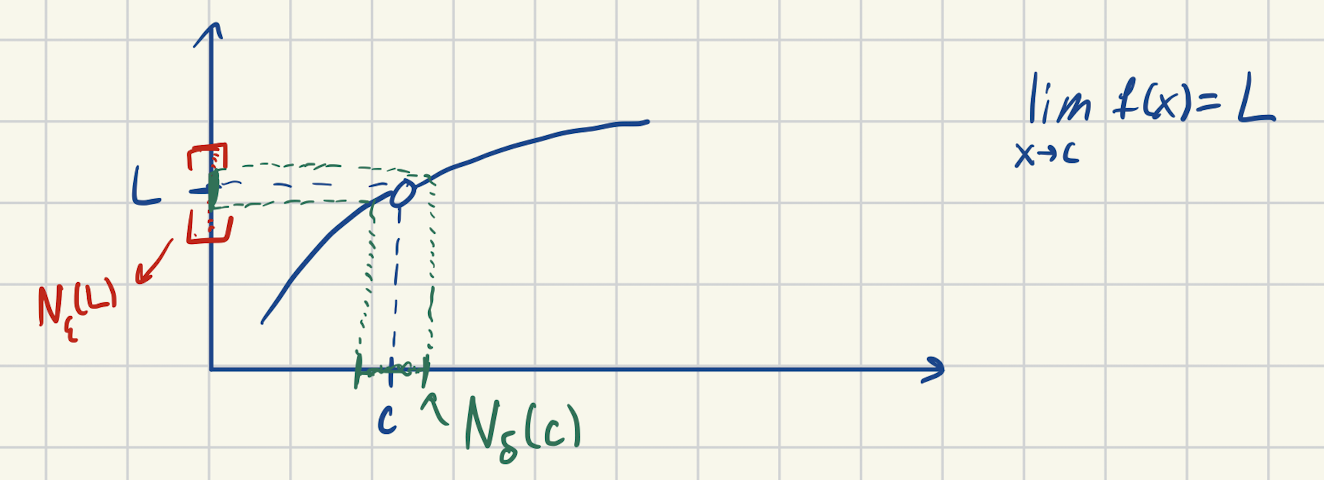
\includegraphics[width=.50\linewidth, center]{/Users/josiahvillarante/GradSchool/Grad-School-Notes/Math230A/Lecture/CH4/images/limit.png}
\end{figure}

\begin{example}
    Let $\begin{cases*}
        f: \R \to \R \\ f(x) = 2x + 5
    \end{cases*}$. Prove that $\lim_{x \to 3}f(x) = 11.$
\end{example}
\begin{proof}
    We want to show $\forall \epsilon > 0 ~\exists \delta > 0 \st \text{if $0 < |x-3| < \delta$, then $|f(x) - 11| < \epsilon$.}$ Let $\epsilon > 0$ be given. Our goal is to find $\delta > 0 \st$
    \begin{equation*}
        \text{if $0 < |x-3| < \delta$ then $|f(x) - L| < \epsilon$.} \tag{$*$}
    \end{equation*}
    \begin{info}
        \begin{align*}
            |f(x) - 11| <\epsilon &\iff |2x+5 - 11| < \epsilon \\ &\iff |2x-6| <\epsilon \\ &\iff 2|x-3| < \epsilon \\ &\iff |x-3| < \frac{\epsilon}{2}.
        \end{align*}
        So, in order to ensure that $(*)$ holds, we need to find $\delta > 0$ such that
        $$\text{if $0 < |x-3| < \delta$, then $|x-3| < \frac{\epsilon}{2}.$}$$ 
    \end{info}
    Let $\delta = \frac{\epsilon}{2}$. For any $x$ with $0 < |x-3| < \delta$, we have
    $$|f(x) - L| = |2x+5 -11| = 2|x-3| < 2 \cdot \delta = 2 \cdot \frac{\epsilon}{2} = \epsilon.$$\qed
\end{proof}

\begin{example}
    Let $\begin{cases*}
        f: \R \to \R \\ f(x) = x^2
    \end{cases*}.$ Prove that $\lim_{x \to 2}f(x) = 4.$
\end{example}
\begin{proof}
    We want to show $\forall \epsilon > 0 ~\exists \delta > 0 \st \text{if $0 < |x-2| < \delta$ then $|f(x) -4| < \epsilon$.}$ Let $\epsilon > 0$ be given. Our goal is to find a number $\delta > 0$ such that
    \begin{equation*}
        \text{if $0 < |x-2| < \delta$ then $|f(x) - 4| < \epsilon$} \tag{$*$}
    \end{equation*}
    \begin{info}
        $$|f(x) - 4| \iff |x^2 -4| < \epsilon \iff |x-2| \cdot |x+2| < \epsilon.$$
        It would be great if we could bound $|x+2|$ with an expression that is easier to work with. Note that for $0 < \delta < 1$ and $0 < |x-2| < \delta$ we have 
        $$|x+2| = |(x-2) + 4| \leq |x-2| + 4 < \delta + 4 \leq 5.$$
        Thus, in order to ensure $(*)$ holds, it is enough to find $0 < \delta \leq 1$ \st
        $$\text{if $0 < |x+2| < \delta$ then $5|x-2| < \epsilon.$}$$
    \end{info}
    Let $\delta = \min \{1, \frac{\epsilon}{5}\}.$ For any $x$ with $0<|x-2|<\delta$ we have 
    $$|f(x) - 4| = |x^2 - 4| = |x-2| \cdot |x+2| < 5 |x-2| \leq 5\left(\frac{\epsilon}{5}\right) = \epsilon.$$
\end{proof}

\begin{example}
    Let $\begin{cases*}
        f: \R \to (\R, \overset{\sim}{d}) \\ f(x) = x^2
    \end{cases*}$ where $\overset{\sim}{d}$ is the discrete metric. Prove that $\lim_{x \to 2}f(x)$ does not exist.
\end{example}
\begin{proof}
    For the sake of contradiction, suppose $\lim_{x \to 2}f(x) = L.$ Then,
    $$\forall \epsilon > 0 ~\exists \delta > 0 \st \text{if $0<|x-2|<\delta$ then $\overset{\sim}{d}(f(x),L)<\epsilon.$}$$
    In particular, for $\epsilon = \frac{1}{2}$,
    $$\exists delta > 0 \st \text{if $0 < |x-2| < \delta$ then $\overset{\sim}{d}(f(x), L) , \frac{1}{2}$.}$$
    Note that
    $$\overset{\sim}{d}(f(x), L) < \frac{1}{2} \implies \overset{\sim}{d}(f(x), L) = 0 \implies f(x) = L.$$
    So,
    $$\exists \delta\ > 0 \st \text{if $2-\delta < x < 2 + \delta, ~x \not = 2,$ then $x^2 = L.$}$$
    Obviously, it is not the case that for all $x\in (2-\delta, 2+\delta), ~x^2$ is equal to a fixed number $L$. Therefore $\lim_{x\to 2}f(x)$ does not exist. \qed
\end{proof}

\begin{theorem}[Sequential Criterion for Limits of Functions] \leavevmode \\
    \label{thm4.2}
    Let $(X,d)$ and $(Y, \overset{\sim}{d})$ be metric spaces, let $E\subseteq X$ be nonempty, and leet $f: X \to Y$. The following are equivalent:
    \begin{enumerate}[$(i)$]
        \item $\lim \limits_{x\to c} f(x) = L$
        \item For all sequences $(a_n)$ in $E \backslash \{c\}$ satisfying $a_n \to c$, we have $f(a_n) \to L$
    \end{enumerate}
\end{theorem}

\begin{proof}
    \begin{description}
        \item[$(i) \implies (ii)$:] \leavevmode \\
        Let $\lim \limits_{x \to c} f(x) = L.$ We want to show that for all $(a_n)$ in $E \backslash \{c\}$ satisfying $a_n \to c$, we have $f(a_n) \to L$. Let $(a_n)$ be a sequence in $E \backslash \{c\}$ such that $a_n \to c$. Our goal is to show that $f(a_n) \to L.$ That is, we want to show
        $$\forall \epsilon > 0 ~\exists N \st \forall n > N ~~\overset{\sim}{d}(f(a_n), L) < \epsilon.$$
        Let $\epsilon > 0$ be given. Our goal is to find $N$ such that
        \begin{equation*}
            \text{if $n > N$ then $\overset{\sim}{d}(f(a_n), L) < \epsilon$} \tag{$*$}
        \end{equation*}
        We have
        \begin{enumerate}[$(I)$]
            \item $\lim \limits_{x \to c} = L \implies \exists \delta > 0 \st \forall x \in \nbhds{\delta}{X}{c} \cap (E \backslash \{c\}) ~~f(x) \in \nbhds{\epsilon}{Y}{L}$
            \item $\lim a_n = c \implies \exists \hat{N} \st \forall n > \hat{N} ~~a_n \in \nbhds{\delta}{X}{c}$
        \end{enumerate}
        We claim that this $\hat{N}$ can be used as the $N$ that we were looking for. Indeed, if we let $N = \hat{N}$, then $(*)$ holds: \\
        For $n > N,$ we have:
        \begin{align*}
            (II) \implies
            \begin{rcases*}
                a_n \in \nbhds{\delta}{X}{c} \\
                a_n \in E \backslash \{c\}
            \end{rcases*}
            &\implies a_n \in \nbhds{\delta}{X}{c} \cap (E \backslash \{c\}) \\
            &\overset{(I)}{\implies} f(a_n) \in \nbhds{\epsilon}{Y}{L}.
        \end{align*} 

        \item[$(ii) \implies (i)$:] \leavevmode \\
        Suppose for all $(a_n) \in E \backslash \{c\}$ satisfying $a_n \to c$, we have $f(a_n) \to L.$ We want to show $\lim \limits_{x \to c} f(x) = L.$ For the sake of contradiction, suppose $\lim \limits_{x \to c} f(x) \not = L$. That is, assume
        $$\sim \left(\forall \epsilon > 0 ~\exists \delta > 0 \st \forall x \in \nbhds{\delta}{X}{c}\cap (E \backslash \{c\}) ~~f(x) \in \nbhds{\epsilon}{Y}{L}\right).$$
        That is,
        $$\exists \epsilon > 0 \st \forall \delta > 0 ~\exists x \in \nbhds{\delta}{X}{c} \cap (E \backslash \{c\}) \st f(x) \not \in \nbhds{\epsilon}{Y}{L}.$$
        So,
        \begin{align*}
            &\delta = 1 &&\exists x_1 \in E\backslash\{c\} \text{ satisfying $d(x_1, c) < 1$ but for which $\overset{\sim}{d}(f(x), L) \geq \epsilon$} \\
            &\delta = \frac{1}{2} &&\exists x_2 \in E\backslash\{c\} \text{ satisfying $d(x_2, c) < \frac{1}{2}$ but for which $\overset{\sim}{d}(f(x), L) \geq \epsilon$} \\
            &\delta = \frac{1}{3} &&\exists x_3 \in E\backslash\{c\} \text{ satisfying $d(x_3, c) < \frac{1}{3}$ but for which $\overset{\sim}{d}(f(x), L) \geq \epsilon$} \\
            \vdots \\
            &\delta = \frac{1}{n} &&\exists x_n \in E\backslash\{c\} \text{ satisfying $d(x_n, c) < \frac{1}{n}$ but for which $\overset{\sim}{d}(f(x), L) \geq \epsilon$}
        \end{align*}
        In this way, we obtain a sequence $(x_n)$ in $E\backslash \{c\} \st x_n \to c$, but for which $\overset{\sim}{d}(f(x_n), L) \geq \epsilon,$ and so $f(x_n) \not \to L.$ This contradicts our assumption.
    \end{description}
    \qed
\end{proof}

\begin{example} \leavevmode \\
    Let $f: \R \backslash \{0\} \to \R$ be defined by $f(x) = \sin\frac{1}{x}.$ Prove that $\lim \limits_{x \to 0} f(x)$ does not exist.
\end{example}

\begin{proof}
    Let $a_n = \frac{1}{2n \pi}, ~b_n = \frac{1}{2n \pi + \pi / 2}.$ Clearly, $(a_n)$ and $(b_n)$ are sequences in $\R \backslash \{0\}$ and $\lim \limits_{n \to \infty} a_n = 0 = \lim \limits_{n \to \infty} b_n.$ However,
    \begin{align*}
        &\lim \limits_{n \to \infty} f(a_n) = \lim \limits_{n \to \infty} \sin \frac{1}{a_n} = \lim \limits_{n \to \infty} \sin (2n\pi) = \lim \limits_{n \to \infty} 0 = 0 \\
        &\lim \limits_{n \to \infty} f(b_n) = \lim \limits_{n \to \infty} \sin \frac{1}{b_n} = \lim \limits_{n \to \infty} \sin (2n\pi + \pi / 2) = \lim \limits_{n \to \infty} 1 = 1 
    \end{align*}
    So, $\lim f(a_n) \not = \lim f(b_n)$. Therefore, $\lim \limits_{x \to 0}\sin \frac{1}{x}$ does not exist.
\end{proof}

\begin{theorem} [Algebraic Limit Theorem for Functions] \leavevmode \\
    \label{thm4.4}
    Let $(x,d)$ be a metric space, $E\subseteq X$ be nonempty, $c \in E'$, and $f,g:E \to \R.$ Assume
    $$\lim \limits_{x \to c} f(x) = L \text{ and } \lim \limits_{x \to c} g(x) = M.$$
    Then
    \begin{enumerate}[$(i)$]
        \item For all $k \in \R ~~\lim \limits_{x \to c}\left(k f(x)\right) = kL$
        \item $\lim \limits_{x \to c} \left(f(x) + g(x)\right) = L+M$
        \item $\lim \limits_{x \to c} \left(f(x) \cdot g(x)\right) = L \cdot M$
        \item $\lim \limits_{x \to c} f(x)/g(x) = L / M,$ provided $M \not = 0$
    \end{enumerate}
\end{theorem}

\begin{proof}
    All of these items follow immediately from the Algebraic Limit Theorem for sequences and the Sequential Criterion for Limits of Functions. \qed
\end{proof}